% TODO: REVIEW MODIFICATION -- chapter title was "Background". Pick your own title; it should name what the chapter covers.
\chapter{Molecular Representations, Models and Label Noise}\label{chap:background}\label{sec2}
% ---- TAKEAWAYS ----
% - A representation turns a molecule into a fixed-length vector of features. Each family captures different information and has its own weakness, so no single one captures everything.
% - Model families differ in how far one wrong label spreads: a tree keeps it in one leaf, an ensemble dilutes it, a neural network can memorize it.
% - Similarity only exists relative to a representation and a coefficient. Activity cliffs and uninformative features break the similar property principle.
% - Real label noise is not independent, identically distributed or Gaussian. It has heavy tails, shared offsets between laboratories and censoring at assay limits.
% - Learning with noisy labels (LNL) covers every method for training on wrong labels. Noise mitigation is the subset that changes the labels. No single method wins.
% - Every split in the thesis is group-aware, never random. NoiseInject supplies the noise and the robustness and uncertainty metrics used in later chapters.
% ---- END TAKEAWAYS ----

% TODO: REVIEW MODIFICATION -- section 2.1 was "Introduction" and held one sentence ("We now break down the two components of QSAR models: molecular representations and predictive models:"). It is now "Overview" and holds the chapter's opening paragraph, as Dablander's Chapter 2 does.
\section{Overview}

% CODE INPUT
% TODO: review, needs manual review -- splits text not yet written; notes in thesis_notes_moved.md
This chapter introduces the concepts to which every later chapter refers. It covers molecular representations, which turn a molecule into a fixed-length vector of features, the model families that learn from them, and the assumption that similar molecules have similar properties, together with the cases in which this assumption breaks down. It then turns to label noise, describing its sources in real assay data, the seven artificial noise conditions used in this thesis and the methods for LNL. The chapter closes with NoiseInject, the package that injects the noise and reports robustness and uncertainty metrics, and with the metrics used throughout.




\section{Molecular Representations in QSAR}
% [notes moved to thesis_notes_moved.md]

% CODE INPUT: first person changed to "we"
% TODO: review, needs manual review
The success of machine learning hinges on the quality of the input data. Although quality can refer to noise, on which most of this work centers, here we mean the type of input that the model receives. Molecular representations provide different features from which QSAR models and noise detection techniques can learn, and Figure~\ref{fig:molecular_representations} shows three of them for a single molecule.

\begin{figure}[!htbp]
	\centering 
	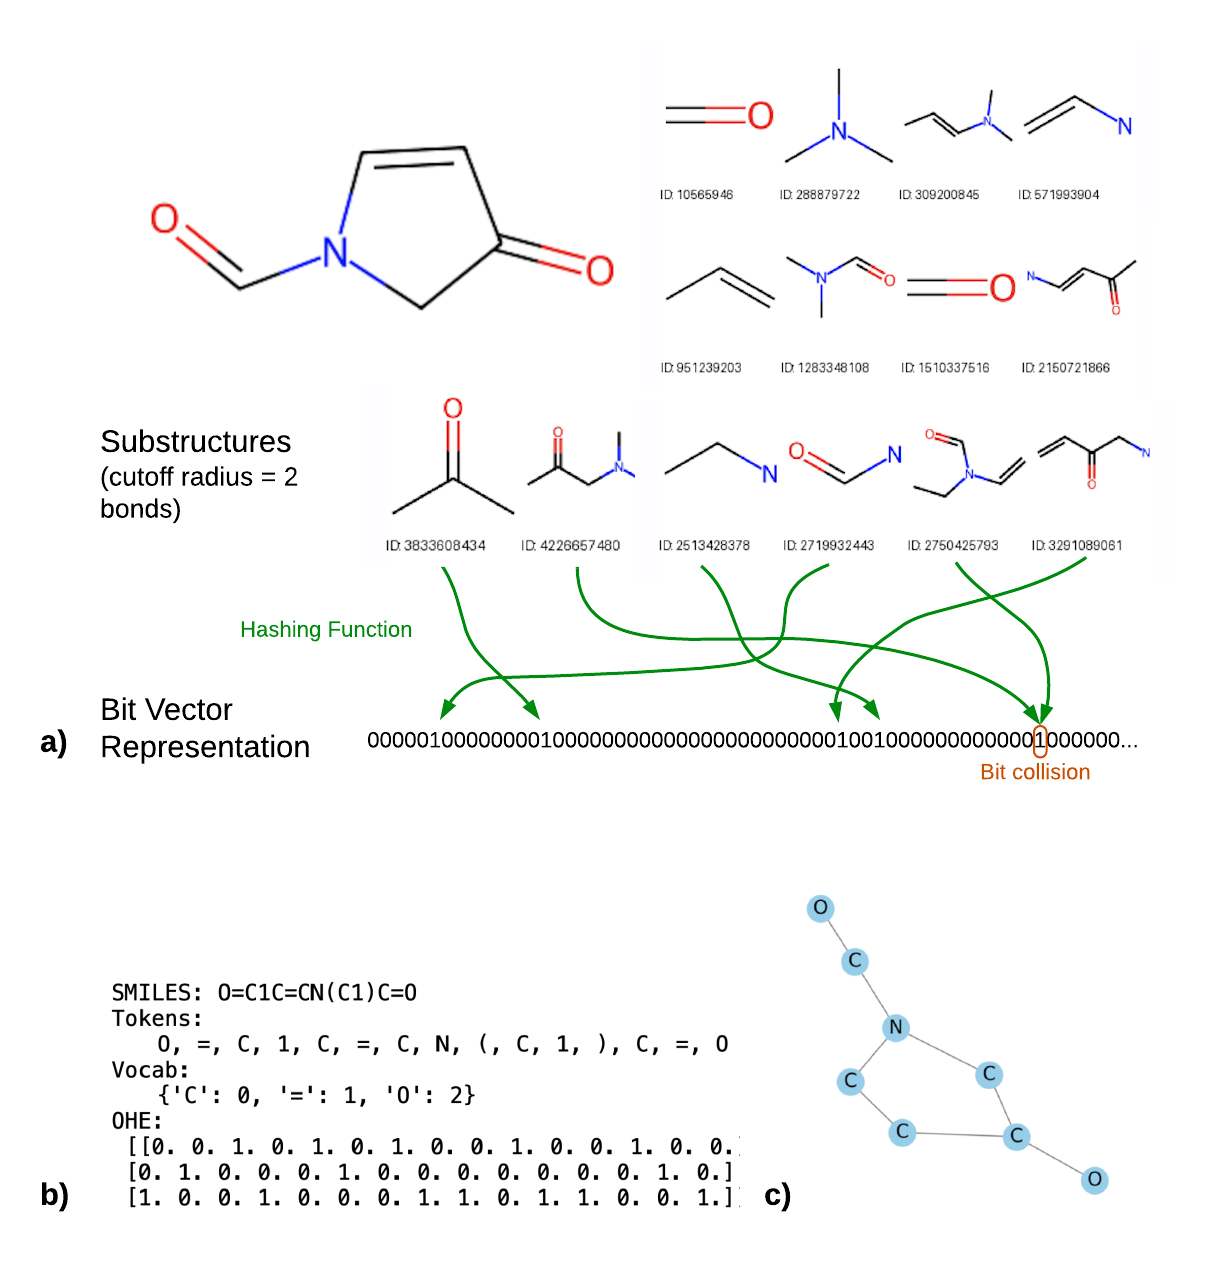
\includegraphics[width=\textwidth,height=0.72\textheight,keepaspectratio]{molecular_representations.png} % TODO: REVIEW MODIFICATION -- was 1.05\textwidth, which ran into the margin	
    \caption[Three representations of one molecule.]{\label{fig:molecular_representations}Three representations of the molecule \lstinline{O=C1C=CN(C1)C=O}. a) ECFP4, in which circular substructures up to a radius of two bonds are hashed (green arrows) to positions in a bit vector, and two substructures can share a position (bit collision, orange). b) Tokenization and one-hot encoding of the SMILES string. c) Molecular graph, with atoms as nodes and bonds as edges.}
\end{figure}

One of the most common and intuitive molecular representations is the Simplified Molecular-Input Line-Entry System (SMILES) string, which consists of a sequence of ASCII characters generated by a fixed set of rules to specify a given chemical identity \citep{Weininger1988}. A common way to use SMILES strings as inputs to QSAR models is to tokenize and one-hot-encode them rather than to use the strings themselves \citep{TeachOpenCADD2023}. The strings are tokenized into atomic branches and symbols and mapped to indices of a vocabulary, and finally converted into binary vectors using one-hot encodings \citep{TeachOpenCADD2023}. This representation, referred to as one-hot-encoded SMILES, allows models to process molecular structures as bit-vector-based fingerprints or as sequences of vectors. Sequence-based models such as recurrent neural networks and transformers have proven to be particularly successful in capturing text semantics within a sequence. When applied to raw or one-hot-encoded SMILES strings, these models can effectively capture the structure of the molecule in its textual representation \citep{TeachOpenCADD2023}. 

Another common representation is the molecular fingerprint, a vector containing information about the properties of the molecule in question. In a typical bit vector-based fingerprint, each bit accounts for the presence (1) or absence (0) of a given chemical feature or substructure \citep{Fassio2022}. One common fingerprint is the Molecular ACCess System (MACCS) key, a substructure key-based fingerprint that encodes predefined atom symbols and properties, as well as bond types \citep{Xie2020}. Another is the Extended Connectivity Fingerprint (ECFP), which encodes local neighborhoods around each atom and bond connectivity in molecules \citep{Xie2020}. ECFPs are typically constructed with a radius of 2, a length of 2048 bits, and active chirality flags. These existing molecular representations are well established and have been quite successful when coupled with QSAR models \citep{CortsCiriano2020, Sabando2021}. They are relatively simple, and as the bits can be mapped back to one or more substructures, they are human-interpretable, and furthermore easy-to-compute. However, they are subject to information loss due to bit collisions, which happens when two different substructures are encoded at the same bit position \citep{Fassio2022}. They are also based on a fixed procedure and are not trainable or adaptable to a particular dataset. Alternative representations that capture different structural, chemical, or physical features are able to overcome these limitations. 

Recent advances have led to the development of new molecular fingerprints. One such method is the Sort \& Slice (SNS) technique, an alternative to hash-based folding for pooling ECFP substructures \citep{sns}. Sort \& Slice begins by sorting all circular substructures in the training set according to their frequency of occurrence. It then ``slices'' away all but the $N$ most frequent substructures, which are subsequently used to generate an $N$-dimensional, bit-collision-free binary fingerprint. This approach solves the ambiguity problem of hashed fingerprints, where multiple substructures might be encoded at the same bit position, making it very interpretable \citep{sns}. Sort \& Slice fingerprints outperform ECFP of diameter four (ECFP4) with standard hash-based folding methods across various molecular property prediction tasks. These experiments consisted of different data splitting techniques, machine learning models, fingerprint diameters, fingerprint dimensions, and atomic invariants \citep{sns}. Furthermore, Sort \& Slice outperformed advanced substructure selection schemes such as filtered fingerprints and mutual information maximization \citep{sns}. 


Neural fingerprints are a category of learned  representations that overcome the fixed, hard-coded nature of traditional fingerprints. Unlike ECFP or MACCS keys, which rely on predefined hashing schemes or substructure catalogs, neural fingerprints train on molecular data to capture chemical information \citep{Jaeger2018, Chithrananda2020}. These representations are the result of deep learning architectures that have learned dense, continuous embeddings which can be used for downstream tasks. 

% TODO: review, needs manual review
Mol2vec, a common neural fingerprint, adapts the Word2vec algorithm from natural language processing (NLP) to molecular substructures \citep{Jaeger2018}. It treats molecules as ``sentences'' and the circular substructures from which ECFPs are built as ``words'', and it learns an embedding for each substructure through unsupervised training, such that chemically similar substructures are mapped to nearby points in the embedding space \citep{Jaeger2018}. The embeddings of all substructures present in a molecule are summed to give a 300-dimensional dense vector that represents the whole molecule \citep{Jaeger2018}. Mol2vec has performed strongly on various QSAR benchmarks, matching or exceeding ECFPs on solubility and bioactivity prediction tasks \citep{Jaeger2018}.

Transformer-based architectures have also been applied to molecular representation learning, similarly stemming from NLP ideas. MolBERT applies a bidirectional transformer to learn molecular representations from SMILES strings through self-supervised pre-training \citep{Fabian2020}. The model has domain-relevant auxiliary adaptations, such as the prediction of calculated physicochemical properties alongside the masked token prediction, to improve the chemical fidelity of the learned embeddings \citep{Fabian2020}. MolBERT demonstrated improvements over traditional fingerprints and graph-based methods on virtual screening and QSAR benchmarks \citep{Fabian2020}. ChemBERTa is another transformer-based approach which pre-trains masked language models on SMILES data from PubChem \citep{Chithrananda2020}.  ChemBERTa uses a tokenization strategy adapted for the SMILES notation, which allows the model to learn representations of atoms and functional groups through self-supervised learning \citep{Chithrananda2020}. Attention visualization reveals that ChemBERTa learns chemically meaningful patterns, with different attention heads specializing in functional groups, ring structures, or SMILES syntax \citep{Chithrananda2020}. ChemBERTa-2, an optimized variant pre-trained on 77 million compounds, achieved even stronger performance than the original ChemBERTa in MoleculeNet benchmarks \citep{Ahmad2022}.

Neural fingerprints provide several advantages over traditional fingerprints. They produce dense continuous vectors that avoid sparseness and information loss from bit collisions \citep{Jaeger2018}. They can also be pre-trained once on large unlabeled datasets and then fine-tuned for specific downstream tasks, opening the door to transfer learning \citep{Chithrananda2020, Fabian2020}. However, these methods are often computationally expensive \citep{Jaeger2018} and due to their black-box nature, they are not as interpretable \citep{Chithrananda2020}, although attention mechanisms offer some interpretability through visualization \citep{Chithrananda2020}.

Beyond fingerprints, physicochemical-descriptor vectors (PDVs) are a class of continuous-value molecular descriptors that encode structural and chemical properties of molecules \citep{Todeschini2009}. Unlike binary fingerprints or graph-based representations, PDVs aggregate atom and bond-level quantities into fixed-length feature vectors that capture a wide variety of information about a molecule and its structure \citep{Mauri2006}. PDVs typically consist of hundreds of properties including constitutional descriptors such as molecular weight, atom and bond counts, and heteroatom ratios; topological indices encoding molecular connectivity patterns; physicochemical properties such as logP (lipophilicity), molar refractivity, and topological polar surface area; and electronic descriptors derived from partial charges and polarizabilities \citep{Todeschini2009, Cherkasov2014}. The \texttt{RDKit} cheminformatics toolkit provides a comprehensive suite of more than 200 molecular descriptors that cover these categories \citep{rdkit}. PDVs are very interpretable; each descriptor has a clear physicochemical meaning \citep{Cherkasov2014}. They are also less computationally expensive than some 3D methods or neural fingerprints, with many descriptors simply requiring a 2D molecular structure without conformer generation or extensive pre-training. This efficiency makes PDVs particularly appropriate for high-throughput applications. Descriptors based on 3D structure can also be used \citep{Mauri2006}.

However, PDVs have limitations. The dimensionality of PDV feature spaces can lead to problems with multicollinearity \citep{Todeschini2009}. This can be mitigated by feature selection or dimensionality reduction techniques \citep{Cherkasov2014}. Additionally, PDVs encode molecular properties as aggregated global features, which may not capture fine-grained structural details such as specific substructure arrangements or local chemical environments, information important for particular endpoints \citep{Mauri2006}.

One of the more intuitive representations is the molecular graph. These graphs can be categorized into 2D and 3D graphs. 2D graphs rely on adjacency matrices that encode topological atom- and bond-level features but leave out geometric properties such as bond angles or torsion, meaning they may fail to capture stereochemistry. 3D graphs incorporate these spatial features, but are often limited by remaining in a single conformation \citep{Zhichun2023}. A standard molecular graph is constructed such that each molecule is represented as $G = (V,E)$ with node features $\mathbf{x}_i$ and edge features $\mathbf{e}_{ij}$. Nodes encode atom type, degree, hybridization, aromaticity, and formal charge; edges encode bond order and conjugation \citep{Zhichun2023}. 

% TODO: review, needs manual review
Another common molecular graph is the standard distance compatibility graph, in which atoms and bonds are mapped to sets of nodes and edges \citep{David2020, Hnig2022}. These graphs are typically 2D objects that encode 3D information such as atomic coordinates, bond angles and chirality \citep{David2020}. Alternative graph representations that incorporate 3D structure and physical interactions include graphs with quantum 3D embeddings, weight alignment graphs, association graphs containing pairs of molecules, and geometric interaction graph neural networks \citep{Hnig2022, yan2023, Yang2023GIGN}. \citet{Du2022} combined 2D and 3D graphs in a zipper-like arrangement, in which the 3D data guarantee precision and completeness by providing unabridged information and the 2D data provide chemical intuition for guidance. Grid-based 3D representations pose a related challenge: atoms localized at single voxels leave the grid too sparse, which leads to poor performance. \citet{Kuzminykh2018} addressed this problem by extending each atom to fill nearby voxels with a wave transformation.
      
These graph representations do not highlight specific substructures or specific arrangements of atoms and bonds within each molecule. The substructures contain functional groups that are related to a range of chemical properties and are potentially involved in downstream tasks related to the function of molecules. \citet{Bouritsas2023} developed graph substructure networks, a topologically aware message passing scheme based on substructure encoding. The method involves encoding structural roles based on the appearance of specific substructures and using them in message passing updates. Since message-passing graph neural networks (GNNs) are at most as powerful as the Weisfeiler--Lehman test, they cannot isolate sufficient features from the graph structure \citep{Bouritsas2023}. Graph substructure networks, on the other hand, capture these substructure-related features. Pretrained GNN encoders can also produce embeddings that capture structural features from unlabeled data \citep{kishimoto2023, ross2022}. 

\section{Models for Molecular Property Prediction}
% [notes moved to thesis_notes_moved.md]

There are a wide variety of model architectures that can be used for QSAR modeling. Starting off with simpler and more explainable models, we have tree-based methods. Decision trees are non-parametric supervised learning algorithms that perform recursive binary partitioning of the feature space \citep{Breiman1984}. A decision tree builds a predictive model by learning a series of if-then rules that recursively split the data based on given feature values, creating a tree  where internal nodes represent decision rules, branches represent the results of those decisions, and leaf nodes contain predicted values or class labels \citep{Breiman1984}. Each recursive split is chosen to maximize  homogeneity within the resulting partitions. For classification, Gini impurity is commonly used and for regression, mean squared error reduction \citep{Breiman1984}.

There are several properties that make decision trees a good foundation for QSAR modeling. First, they handle non-linear relationships between molecular descriptors and target properties without requiring explicit feature engineering or transformation \citep{Breiman1984}. They also do not make assumptions about the underlying distribution of the data, making them robust to violations of parametric assumptions that can limit linear regression or other classical methods \citep{Svetnik2003}. 

Decision trees handle data in a ``contributory'' rather than ``consensus'' manner. In consensus methods such as linear regression or neural networks, every data point influences the prediction at every other point in the feature space. Tree-based methods make predictions based on the subset of training samples that fall into the same leaf node as the test point \citep{Breiman1984}. This mechanism essentially quarantines outliers in their respective leaf nodes, limiting their impact on predictions for samples in other regions or chemical domains. 

% TODO: review, needs manual review
Individual decision trees tend to have high variance and often overfit, particularly at large depths \citep{Breiman1984}. Small modifications made to the training data can result in large differences in the structure of the tree, resulting in unstable predictions \citep{Breiman2001}. Ensemble methods are used to counteract this instability, aggregating predictions from many trees. Random forests (RFs) aggregate predictions from trees trained on bootstrap samples of data with random subsets of features at each split \citep{Breiman2001}. Bootstrapping ensures that each tree is trained on a slightly different subset of data, which effectively reduces the influence of any individual sample \citep{Breiman2001}. This is especially beneficial with noisy samples. The selection of random features at every node decorrelates the trees, preventing systematic biases from propagating through the ensemble \citep{Breiman2001}. The aggregation of trees further prevents overfitting to noise by smoothing out prediction errors from individual noisy labels. 

% TODO: review, needs manual review
Neural networks (NNs), a very popular family of models, can also be used for QSAR. An NN is a system of interconnected nodes which learn by passing information through its layers. There are weights and biases attached to the nodes and various other parameters which the model optimizes to minimize the difference between the predicted output and the actual target value. During training, the network parameters are updated using backpropagation, in which gradients of the loss function with respect to each weight are propagated backward through the network \citep{Rumelhart1986}. The structure of these networks and the hyperparameters used depend on the type of NN. In QSAR, one of the most commonly used architectures is the multilayer perceptron (MLP), a NN containing fully-connected layers with non-linear activation functions which transforms molecular feature vectors (i.e., fingerprints, descriptors) into a property or activity prediction \citep{Ma2015}.

For molecular property prediction, it is recommended that architectures use 2--3 hidden layers with 128--512 units each, rectified linear unit (ReLU) activations, and dropout regularization to prevent overfitting. Training is performed using backpropagation with gradient descent optimizers such as Adam, to minimize a loss function (mean squared error for regression, cross-entropy for classification) on batches of training data \citep{wu2018}. 

% TODO: review, needs manual review
However, NN performance on QSAR-related tasks has been very mixed. They are often outperformed by more traditional methods: decision trees and related ensemble models tend to perform better on smaller datasets and to overfit less \citep{Baskin2008, Koutsoukas2017}. Their complexity and use of gradients make them prone to label memorization \citep{Zhang2017}, which in the context of noise is problematic, as it means that models may memorize the noise themselves. Although models that are memorizing labels may initially appear to have strong predictive performance, they cannot generalize to out-of-distribution samples properly and often provide inaccurate uncertainty estimates. Various approaches have been proposed to improve neural network robustness to label noise, including noise-robust loss functions \citep{Song2022}, confident learning to identify mislabeled examples \citep{Northcutt2021}, and regularization techniques such as mixup \citep{Zhang2018mixup} or label smoothing \citep{Szegedy2015}. 

% TODO: review, needs manual review
All the models up to this point have assumed a vector-based input. Molecular graphs, on the other hand, require different types of predictive modeling. Two standard ML methods on molecular graphs include Graph Convolutional Networks (GCNs) and Graph Isomorphism Networks (GINs). GCNs apply the concept of convolution to graph-structured data. Instead of operating on grid-based data, such as images, GCNs aggregate information from neighbors of a node to update its representation \citep{TeachOpenCADD2023, Xu2019}. In contrast, GINs address the limitations in GCNs’ ability to differentiate between non-isomorphic graphs. Unlike GCNs, which normalize and weight the sum of neighboring node features, GINs use a simple sum followed by a trainable MLP, giving the model flexibility to learn complex transformations of node features. The GIN model’s design is informed by the Weisfeiler--Lehman test for graph isomorphism, enabling it to distinguish between molecular graphs that are structurally similar but differ in subtle ways \citep{TeachOpenCADD2023, Xu2019}. This makes GINs a candidate for modeling activity cliffs (Section~\ref{sec:mol_similarity}), where small variations in molecular structure can lead to significant changes in chemical or biological activity \citep{TeachOpenCADD2023}. 


\subsection{Tree Ensembles}
% [notes moved to thesis_notes_moved.md]


% TODO: review, needs manual review
Quantile Regression Forests (QRFs) extend RFs by holding the distribution of training labels in each leaf and computing quantiles over all trees \citep{Meinshausen2006}.

% TODO: review, needs manual review
Gradient boosting methods such as eXtreme Gradient Boosting (XGBoost) sequentially fit trees to the residuals of previous iterations, progressively reducing the prediction error \citep{Chen2016, Mustapha2016, Tian2022}. Other gradient-boosted tree ensembles include Light Gradient-Boosting Machine (LightGBM) \citep{ke2017lightgbm}, and Natural Gradient Boosting (NGBoost) \citep{Duan2020}. NGBoost extends deterministic gradient boosting by treating the parameters of a chosen parametric distribution as regression targets and learns them through boosting with a natural gradient update rule \citep{Duan2020}.


\subsection{Support Vector Machines}
% [notes moved to thesis_notes_moved.md]
% - Answer to your TODO: Chapter 3 reports how the SVM holds up under each noise condition. Point there; do not restate the numbers.

% TODO: review, needs manual review
Support vector machines (SVMs) are a well-established baseline in QSAR modeling, mapping inputs into a high-dimensional feature space in which, for classification, a maximum-margin hyperplane separates the classes \citep{Vapnik1995, Svetnik2003}.
% TODO: anything interesting to say on SVMs? Background? promising results with noise (it's actually one of the top performing in my results)
% Limitations - compute too high on large N

% CODE INPUT
% TODO: review, needs manual review
Support vector regression fits a function that is as flat as possible while keeping training errors small \citep{Vapnik1995, Smola2004}. It uses the $\epsilon$-insensitive loss, under which errors smaller than $\epsilon$ cost nothing and larger errors cost their size minus $\epsilon$. A constant $C$ trades flatness against tolerance of large errors \citep{Cortes1995}. The features enter the model only through the kernel. With the radial basis function (RBF) kernel, the kernel is a function of the Euclidean distance, so every feature enters every distance. In Chapter~\ref{chap:robustness} the continuous representations are standardized and the binary fingerprints are used as built. Three properties of the method suggest robustness to label noise. Errors inside the $\epsilon$ tube change nothing, the loss outside the tube grows linearly rather than quadratically, and the weight of each molecule is capped at $C$ \citep{Smola2004}. Under simulated experimental error, the RBF-kernel SVM degraded smoothly and linearly \citep{Cortes2015}, and Chapter~\ref{chap:robustness} reports how it holds up under each of our noise conditions. Its main limitation is computational cost, because training operates on a kernel matrix that grows with the square of the number of training molecules \citep{Chang2011}.


\subsection{Gaussian Processes}
% [notes moved to thesis_notes_moved.md]

Gaussian processes (GPs) are a non-parametric class of models that use a kernel to produce a Gaussian predictive distribution over every data point \citep{Obrezanova2007, Rasmussen2005}. One of the major limitations of using GPs in practice is computational scaling; inference has $O(N^3)$ time complexity and $O(N^2)$ memory, where $N$ is the number of training points \citep{Rasmussen2005}. This can be mitigated with sparse GP approximations, but these introduce approximation error and can be more difficult to tune \citep{quinonero2005}.


% TODO: review, needs manual review
The \texttt{Gauche} framework \citep{gauche} defines kernels for strings, fingerprints, and graphs that operate on a range of widely used molecular representations. The Tanimoto kernel \citep{Ralaivola2005, moss2020} is defined for binary vectors $\mathbf{x}, \mathbf{x}' \in \{0, 1\}^d$ for $d \geq 1$ as:

% CODE INPUT: $$...$$ changed to an equation environment with a label, so Chapter 4 can refer to it. Needs review.
\begin{equation}
k_{\text{Tanimoto}}(\mathbf{x}, \mathbf{x}') := \sigma_f^2 \cdot \frac{\langle \mathbf{x}, \mathbf{x}' \rangle}{\|\mathbf{x}\|^2 + \|\mathbf{x}'\|^2 - \langle \mathbf{x}, \mathbf{x}' \rangle},
\label{eq:tanimoto_kernel}
\end{equation}

where $\|\cdot\|$ represents the Euclidean norm \citep{gauche}. 

% TODO: review, needs manual review
The RBF kernel is defined for
$\mathbf{x}, \mathbf{x}' \in \mathbb{R}^d$ as:

\begin{equation}
k_{\text{RBF}}(\mathbf{x}, \mathbf{x}') := \sigma_f^2 \cdot \exp\left(-\frac{\|\mathbf{x} - \mathbf{x}'\|^2}{2\ell^2}\right),
\end{equation}

where $\ell$ is the lengthscale and $\sigma_f^2$ the signal variance, which scales both kernels.


\subsection{Bayesian Neural Networks}
% [notes moved to thesis_notes_moved.md]
% - Answer to your TODO: keep the paragraph. It is the only definition of the two parts in the thesis, and Chapter 3 uses both for every probabilistic model.

NNs are often deterministic; however, they can be transformed into probabilistic models (Figure~\ref{fig:bayesian_transformation}).

\begin{figure}[!htbp]
    \centering
    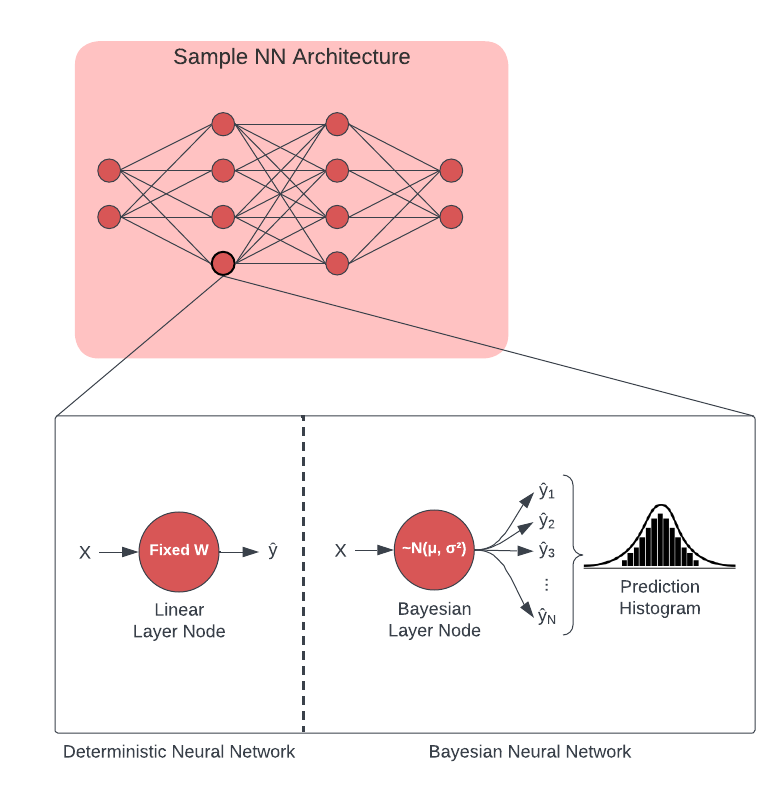
\includegraphics[width=0.85\textwidth,height=0.72\textheight,keepaspectratio]{bayesian_transformation.png}
    \caption[Nodes of a deterministic and a Bayesian neural network.]{One node of a deterministic and of a Bayesian neural network. The deterministic node (bottom left) applies a fixed weight $W$ and returns one prediction $\hat{y}$. The Bayesian node (bottom right) draws its weight from $\mathcal{N}(\mu, \sigma^2)$, so repeated predictions $\hat{y}_1, \dots, \hat{y}_N$ form a histogram.}
    \label{fig:bayesian_transformation}
\end{figure}

Unlike standard deterministic ML methods, Bayesian methods model distributions over predictions using Bayes' rule, allowing for the quantification of uncertainty within parameters and labels. Bayesian methods treat the model parameters as random variables with distributions. Uncertainty can also be estimated from other non-deterministic methods, including deep ensembles \citep{lakshminarayanan2017}, bootstrap modeling \citep{palmer2022}, and federated learning \citep{Hanser2023}.

% TODO: this paragraph may need to go
Epistemic uncertainty is model-driven and can be reduced by collecting either more or higher quality training data. Aleatoric uncertainty is data-driven and reflects the intrinsic noise in the labels.

\section{Molecular Similarity and Activity Cliffs}\label{sec:mol_similarity}
% [notes moved to thesis_notes_moved.md]
% - Answer to your TODO on the bib: the entries are in refs.bib. Still to fix: Dablander2023 lists "Michael Dablander"; it should be Markus Dablander.

% TODO: hand edit
% TODO: review, needs manual review
Much of cheminformatics rests on the similar property principle, which states that structurally similar molecules tend to have similar properties \citep{Johnson1990, vanTilborg2022}.
One of its clearest applications is nearest-neighbor prediction, which appears across cheminformatics workflows and, in this thesis, in the kernels used by GPs and at the basis of many noise identification algorithms.

% TODO: review, needs manual review
The difficulty with this principle is that similarity is defined only relative to a similarity measure, which is fixed by the choice of representation and
coefficient \citep{Maggiora2014}. There is no standard definition of similarity between molecules, especially when different molecular embeddings are handled in a computational setting. Two molecules that are near-identical under a substructure fingerprint may be far apart under a PDV, and \citet{Maggiora2014} caution that quantified similarity can be over-interpreted in this way.

% CODE INPUT: formula added so that Chapter 4's argument about distances has its starting point here
The most common measure for binary fingerprints is the Tanimoto coefficient \citep{Bajusz2015}. For two molecules with fingerprints $\mathbf{x}, \mathbf{x}' \in \{0,1\}^d$,
\begin{equation}
T(\mathbf{x}, \mathbf{x}') = \frac{\sum_{j=1}^{d} x_j x'_j}{\sum_{j=1}^{d} x_j + \sum_{j=1}^{d} x'_j - \sum_{j=1}^{d} x_j x'_j},
\label{eq:tanimoto}
\end{equation}
which is the number of bits set in both molecules divided by the number of bits set in either. Continuous representations are instead compared with a distance, most often the Euclidean distance $\sqrt{\sum_{j=1}^{d}(x_j - x'_j)^2}$. Both measures are sums over the features, and neither weighs a feature by its relation to the property. In the Tanimoto coefficient, a bit that is off in both molecules contributes nothing, whereas every bit that is set in either molecule counts. In the Euclidean distance, every feature that differs between the two molecules counts. Chapter~\ref{chap:flaws} returns to this point (Equation~\ref{eq:distance_split}).

% TODO: review, needs manual review
Distance-based reasoning relies on the assumption that the data embeddings contain quality information. When the labels are corrupted or few features relate to the property, similarity scores are dominated by features that carry no information about it, and the assumption that similar molecules have similar properties breaks down. % TODO: REVIEW MODIFICATION -- removed a doubled "et al." and a repeated citation of Bajusz2015.
\citet{Bajusz2015} found that while the Tanimoto coefficient can be effective with binary fingerprints, changing the similarity formula yields minimal improvement if the underlying representation is weak.
This problem is further complicated by activity cliffs, defined below, which potentially contain the most important information for model prediction but can be confused with noise. Another barrier to distance-based reasoning is persistent noise across labels. The task of trying to determine if a molecule's value matches that of its neighbors becomes a lot harder when all of the neighbors have some form of noise as well.

There are many downstream tasks which rely on the concept of similarity. The second half of this thesis relies on many such tasks, and as such focuses on identifying representations that agree with this principle. 


% TODO: review, needs manual review
The sharpest failure of the similar property principle is the activity cliff, a pair of structurally similar molecules with a large difference in potency that is produced by a small
chemical change \citep{Maggiora2006, Stumpfe2012}. Activity cliffs inherit the measure dependence of the principle they violate, and there is no widely accepted definition of one
\citep{vanTilborg2022}. The MoleculeACE benchmark \citep{vanTilborg2022} makes this choice explicit. A pair is considered highly similar if its similarity exceeds 90\% under at least one of
three measures, namely the Tanimoto coefficient on ECFPs, the Tanimoto coefficient on scaffold fingerprints and a scaled Levenshtein distance on SMILES strings. Such a pair forms a cliff if
the two molecules also differ tenfold or more in $K_i$ or EC$_{50}$ \citep{vanTilborg2022}. This soft consensus over three measures is used because each measure captures only part of the
underlying chemistry. Across the thirty MoleculeACE targets, cliff compounds account for between 7\% and 52\% of a dataset \citep{vanTilborg2022}.

% TODO: review, needs manual review
Dimensionality itself poses a further difficulty. \citet{Aggarwal2001} show that as the number of dimensions grows, the distances to the nearest and to the furthest
point become increasingly similar, so that pairwise distances become progressively less discriminative. Molecular representations are routinely high-dimensional and sparse, and when a
large proportion of their dimensions carry no information relevant to the property being modeled, distances computed over them are dominated by those uninformative dimensions.


% TODO: make changes to bib

\section{Noise in Molecular Data}
% [notes moved to thesis_notes_moved.md]

% TODO: review, needs manual review
Real-world cheminformatics datasets contain label noise arising from multiple sources across the drug discovery pipeline, and modeling experimental noise properly requires first understanding where it comes from.

% moved here from the start of the Models section (2026-09-30)
% TODO: review, needs manual review
One key issue with QSAR models is the standard assumption that labels represent true values. Most ML models rely on the assumption that the training data is, in fact, an accurate reflection of the population. Therefore, they treat these potentially noisy labels as exact point values rather than as draws from a distribution, which opens the door to overfitting to noise and giving unduly optimistic assessments of the models.

Studies involving noise, and specifically the quantification of noise robustness, typically approach label noise by adding independent, zero-mean, Gaussian error to the labels. However, there is evidence that noise from experimental assays takes on different forms. \citet{Kruger2012} rejected normality of bioactivity differences by Anderson-Darling test and fitted a Laplace distribution instead. \citet{Kalliokoski2013} examined the widest disagreements among 16,844 pairs of repeat pIC$_{50}$ measurements and found that in almost all cases, the wide gap between repeat values was due to annotation error rather than to an imprecise assay.

% TODO: review, needs manual review
\citet{Kolmar2021} examined the predictive limits of QSAR in the presence of noise and showed that, by learning the underlying trends rather than fitting the noise, models can make predictions that are more accurate than their own training labels. They assumed that experimental noise is Gaussian, arguing from the central limit theorem that measurements aggregated over multiple independent error sources follow a Gaussian distribution. \citet{Heid2023}, however, used mean-variance estimation and bias-variance decomposition to show that noise can be tied to specific properties of the molecules, such as their structure. For example, nitrogen-containing functional groups introduce measurement deviations, which implies the presence of systematic noise.

% TODO: review, needs manual review (last sentence adapted from paper.tex to point to Chapter 3)
% TODO: review, needs manual review
Beyond just the distribution, the assumptions of independence and zero mean may fail as well. \citet{Bentz2013} examined P-glycoprotein transport measurements across 23 laboratories and found that $62\%$ of the variance in log efflux ratio was due to differences between laboratories. When data are pooled from different sources, each source can carry a shared offset. These sources usually contain families of related compounds, breaking the independence assumption. The zero-mean assumption is not assured either, especially when true values fall above or below an assay's detection limit, called censoring. \citet{Svensson2025} count censored labels in fifteen industrial assays, of which thirteen carry censored labels and eight sit between a quarter and two thirds censored. Chapter~\ref{chap:robustness} tests noise conditions that vary the distribution, the correlation, and the bias of injected error separately, at a matched quantity of noise for every condition except censoring.

% TODO: REVIEW MODIFICATION -- the six paragraphs on noise sources are now Table tab:noise_sources. Every example and citation in the table is from those paragraphs; originals kept below.
% Assay-related variability represents a primary source of label noise in bioactivity data. High-throughput screening assays are often laden with errors from physical phenomena such as edge effects, where compounds in wells exhibit different activities at plate boundaries due to evaporation or temperature gradients \citep{Macarron2011}. Other examples include compound carryover between wells, incomplete liquid transfers, and air bubbles  \citep{Inglese2006}.  Detection reagents or unstable compounds can degrade over time, which leads to drift within a single plate run. This turns into heteroscedastic noise correlated with plate position or read time \citep{Brideau2003}.
% 
% Instrument calibration and detection limits can impact measurement accuracy. Spectrophotometric assays near detection limits exhibit higher relative error, such that signal-to-noise ratios degrade for weak binders \citep{Zhang1999}. Fluorescence quenching by test compounds introduces a systematic bia in fluorescence-based assays, resulting in false negatives for potent inhibitors that accidentally get absorbed at emission wavelengths \citep{Simeonov2008}. Radiometric assays require background subtraction and decay corrections that accumulate error, particularly for low-activity compounds where the signal barely exceeds background \citep{Zhang1999}.
% 
% Another source of noise is biological variability. Even minor variations in cell culture conditions such as seeding density, plating efficiency, growth rate, and cell cycle distribution have the potential to affect downstream tasks such as cell metabolism and drug responsiveness. Even serum properties may introduce variability \citep{Hatzis2014}. The speed of cell culture passages is even found to be a significant factor in behavior \citep{Postnikova2018}. 
% 
% Data aggregation across multiple sources compounds these individual error sources. Common databases like ChEMBL, BindingDB, and PubChem aggregate measurements from hundreds of laboratories using a diverse set of protocols, compound purities, and quality control standards \citep{Gaulton2017, Gilson2016}. The $K_i$ or IC$_{50}$ values from the same compound-target pair with between 10 and 20 reported values, often end up spanning two orders of magnitude apart, making it challenging to identify the underlying ground truth \citep{Kramer2012}. All the sources of error mentioned above regarding inconsistent experimental protocols cannot be distinguished easily from the genuine underlying value without extensive, and often unrealistic amounts of metadata \citep{Fourches2016}.
% 
% 
% Federated datasets, a method of data aggregation centered around privacy protection, presents a particularly challenging situation for noise. In pharmaceutical research and beyond, companies often want to merge collective information without exposing proprietary data to competitors. One example of such platforms is Lhasa Limited's federated learning platform Effiris. Teacher models are first trained separately on confidental data, and then used to label a shared public chemical data set. Those results are consolidated into a federated student model \citep{Bassani2023}. While this is an effective approach of protecting intellectual property, it introduces additional label noise through the prediction errors of all the teacher models. There also exists aleatoric uncertainty from the underlying experimental measurements, many of which likely come from differing protocols, resulting in compounding label noise. 
% 
% Beyond the experimental setups, annotation errors in the data itself can arise from mis-registered structures, incorrect stereochemistry assignments, and salt form ambiguity \citep{Williams2017}. Public databases are estimated to contain 1-5\% structure errors from incorrect SMILES parsing, tautomer misassignment, or manual transcription mistakes during data entry \citep{Young2008}. Ambiguous protonation states and counterions create representation-level noise where chemically distinct samples are classified as the same \citep{Bento2020}.

Label noise enters bioactivity data at every step from the assay plate to the database. Table~\ref{tab:noise_sources} lists these sources, with examples of each and the kind of error each tends to produce. The kind of error describes how the error is distributed across molecules, which is the property that the noise conditions in Section~\ref{sec:noise_injection} vary.
\begin{table}[htbp]
\centering
\small
\begin{adjustbox}{max width=\textwidth,max totalheight=0.78\textheight}
\begin{tabular}{@{}P{0.16\linewidth}P{0.46\linewidth}P{0.30\linewidth}@{}}
\toprule
\textbf{Source} & \textbf{Example} & \textbf{Kind of Error} \\
\midrule
Assay & Edge effects at plate boundaries from evaporation or temperature gradients \citep{Macarron2011}; carryover between wells, incomplete liquid transfers and air bubbles \citep{Inglese2006}; reagents or compounds degrading during a run \citep{Brideau2003} & Error that varies with plate position or read time \\
Instrument & Higher relative error near a detection limit \citep{Zhang1999}; fluorescence quenching by the test compound \citep{Simeonov2008}; background subtraction in radiometric assays \citep{Zhang1999} & Larger error for weak binders; a systematic bias; labels clipped at the limit \\
Biology & Seeding density, growth rate, cell cycle and serum properties \citep{Hatzis2014}; passage speed \citep{Postnikova2018} & Variation between repeats of the same experiment \\
Aggregation across sources & ChEMBL, BindingDB and PubChem pool hundreds of laboratories \citep{Gaulton2017, Gilson2016}; $K_i$ or IC$_{50}$ values for one compound--target pair spanning two orders of magnitude \citep{Kramer2012} & An offset shared by each laboratory or source, hard to separate from the true value without metadata \citep{Fourches2016} \\
Federated learning & Teacher models label a shared public set, and a student model learns from those labels \citep{Bassani2023} & The teachers' prediction errors on top of the measurement error \\
Annotation & Mis-registered structures, wrong stereochemistry and salt forms \citep{Williams2017}; 1--5\% structure errors in public databases \citep{Young2008}; ambiguous protonation states and counterions \citep{Bento2020} & A label attached to the wrong molecule; distinct molecules merged \\
\bottomrule
\end{tabular}
\end{adjustbox}
\caption[Sources of label noise in bioactivity data.]{Sources of label noise in bioactivity data, with reported examples and the kind of error each source produces.}
\label{tab:noise_sources}
\end{table}

% CODE INPUT: first person changed to "we"
% TODO: review, needs manual review
These sources of noise can interact with one another and produce errors that a simple Gaussian does not describe. Real-world noise, unlike the independent Gaussian noise usually injected in robustness studies, is neither independent, identically distributed, nor symmetric \citep{Heid2023}. We address this complexity by examining several ways of both modeling noise and adding it to datasets.

% TODO: review, needs manual review
Although the general assumption in much of the noise analysis and mitigation literature is that noise, specifically label noise, will have a negative effect on the model, this is not necessarily the case. There are multiple instances of using noise as a method of regularization. Although not the optimal approach to counteracting overfitting in linear regression, adding artificial noise to labels is considered a form of regularization \citep{Ullah2024}. Furthermore, adding artificial noise drawn from a Gaussian distribution to the activation layers of a neural network is considered another form of regularization \citep{Camuto2021}. Label noise may therefore act as a regularizer in some QSAR and quantitative structure--property relationship models.

\subsection{Artificial Noise Injection}\label{sec:noise_injection}
% [notes moved to thesis_notes_moved.md]
% - Answer to your TODO on the 20\%: no published estimate exists of how large a share of a dataset a difference between laboratories affects. So 20\% of molecules was chosen, not sourced. Whole scaffold families are drawn until about 20\% of the split is covered.

% TODO: review, needs manual review
To evaluate the robustness of QSAR models against label noise, we inject artificial noise into the training labels, while test labels remain free of noise. Validation labels receive noise of the same type and quantity as the training labels, drawn independently. The noise conditions are designed to mimic particular features of real experimental noise. The clean target label $y_i$ is replaced by a noisy label $\tilde{y}_i = y_i + \epsilon_i$, where $\epsilon_i$ is the artificial noise injected at the index $i$, the value of which is determined by a specified noise strategy.

% TODO: REVIEW MODIFICATION -- the paragraph listing the seven conditions is now a two-sentence lead-in; the list moved into Table tab:noise_conditions. Original kept below.
% We explored seven methodologies of adding noise, referred to as noise conditions (Figure~\ref{fig:noise_conditions}). Three vary the shape of the distribution from which the error is drawn. These shapes include Gaussian, Student-$t$ with $\nu = 5$, and Laplace distributions. Two conditions concentrate error on specific subset of molecules; outlier isolates a random tenth of them and grouped-wider concentrates on Bemis--Murcko scaffold families. Group shifted also applies noise to scaffolds, but instead gives each scaffold its own offset rather than a wider error. The seventh, censoring, sets a limit such that every label extends past that limit is reassigned to the limit itself. 
We explored seven ways of adding noise, which we refer to as noise conditions and which are illustrated in Figure~\ref{fig:noise_conditions} and summarized in Table~\ref{tab:noise_conditions}. Three conditions vary the shape of the distribution from which the error is drawn, and three concentrate the error on some molecules or share it within Bemis--Murcko scaffold families. The seventh condition, censoring, clips labels at a limit.

\begin{figure}[!htbp]
\centering
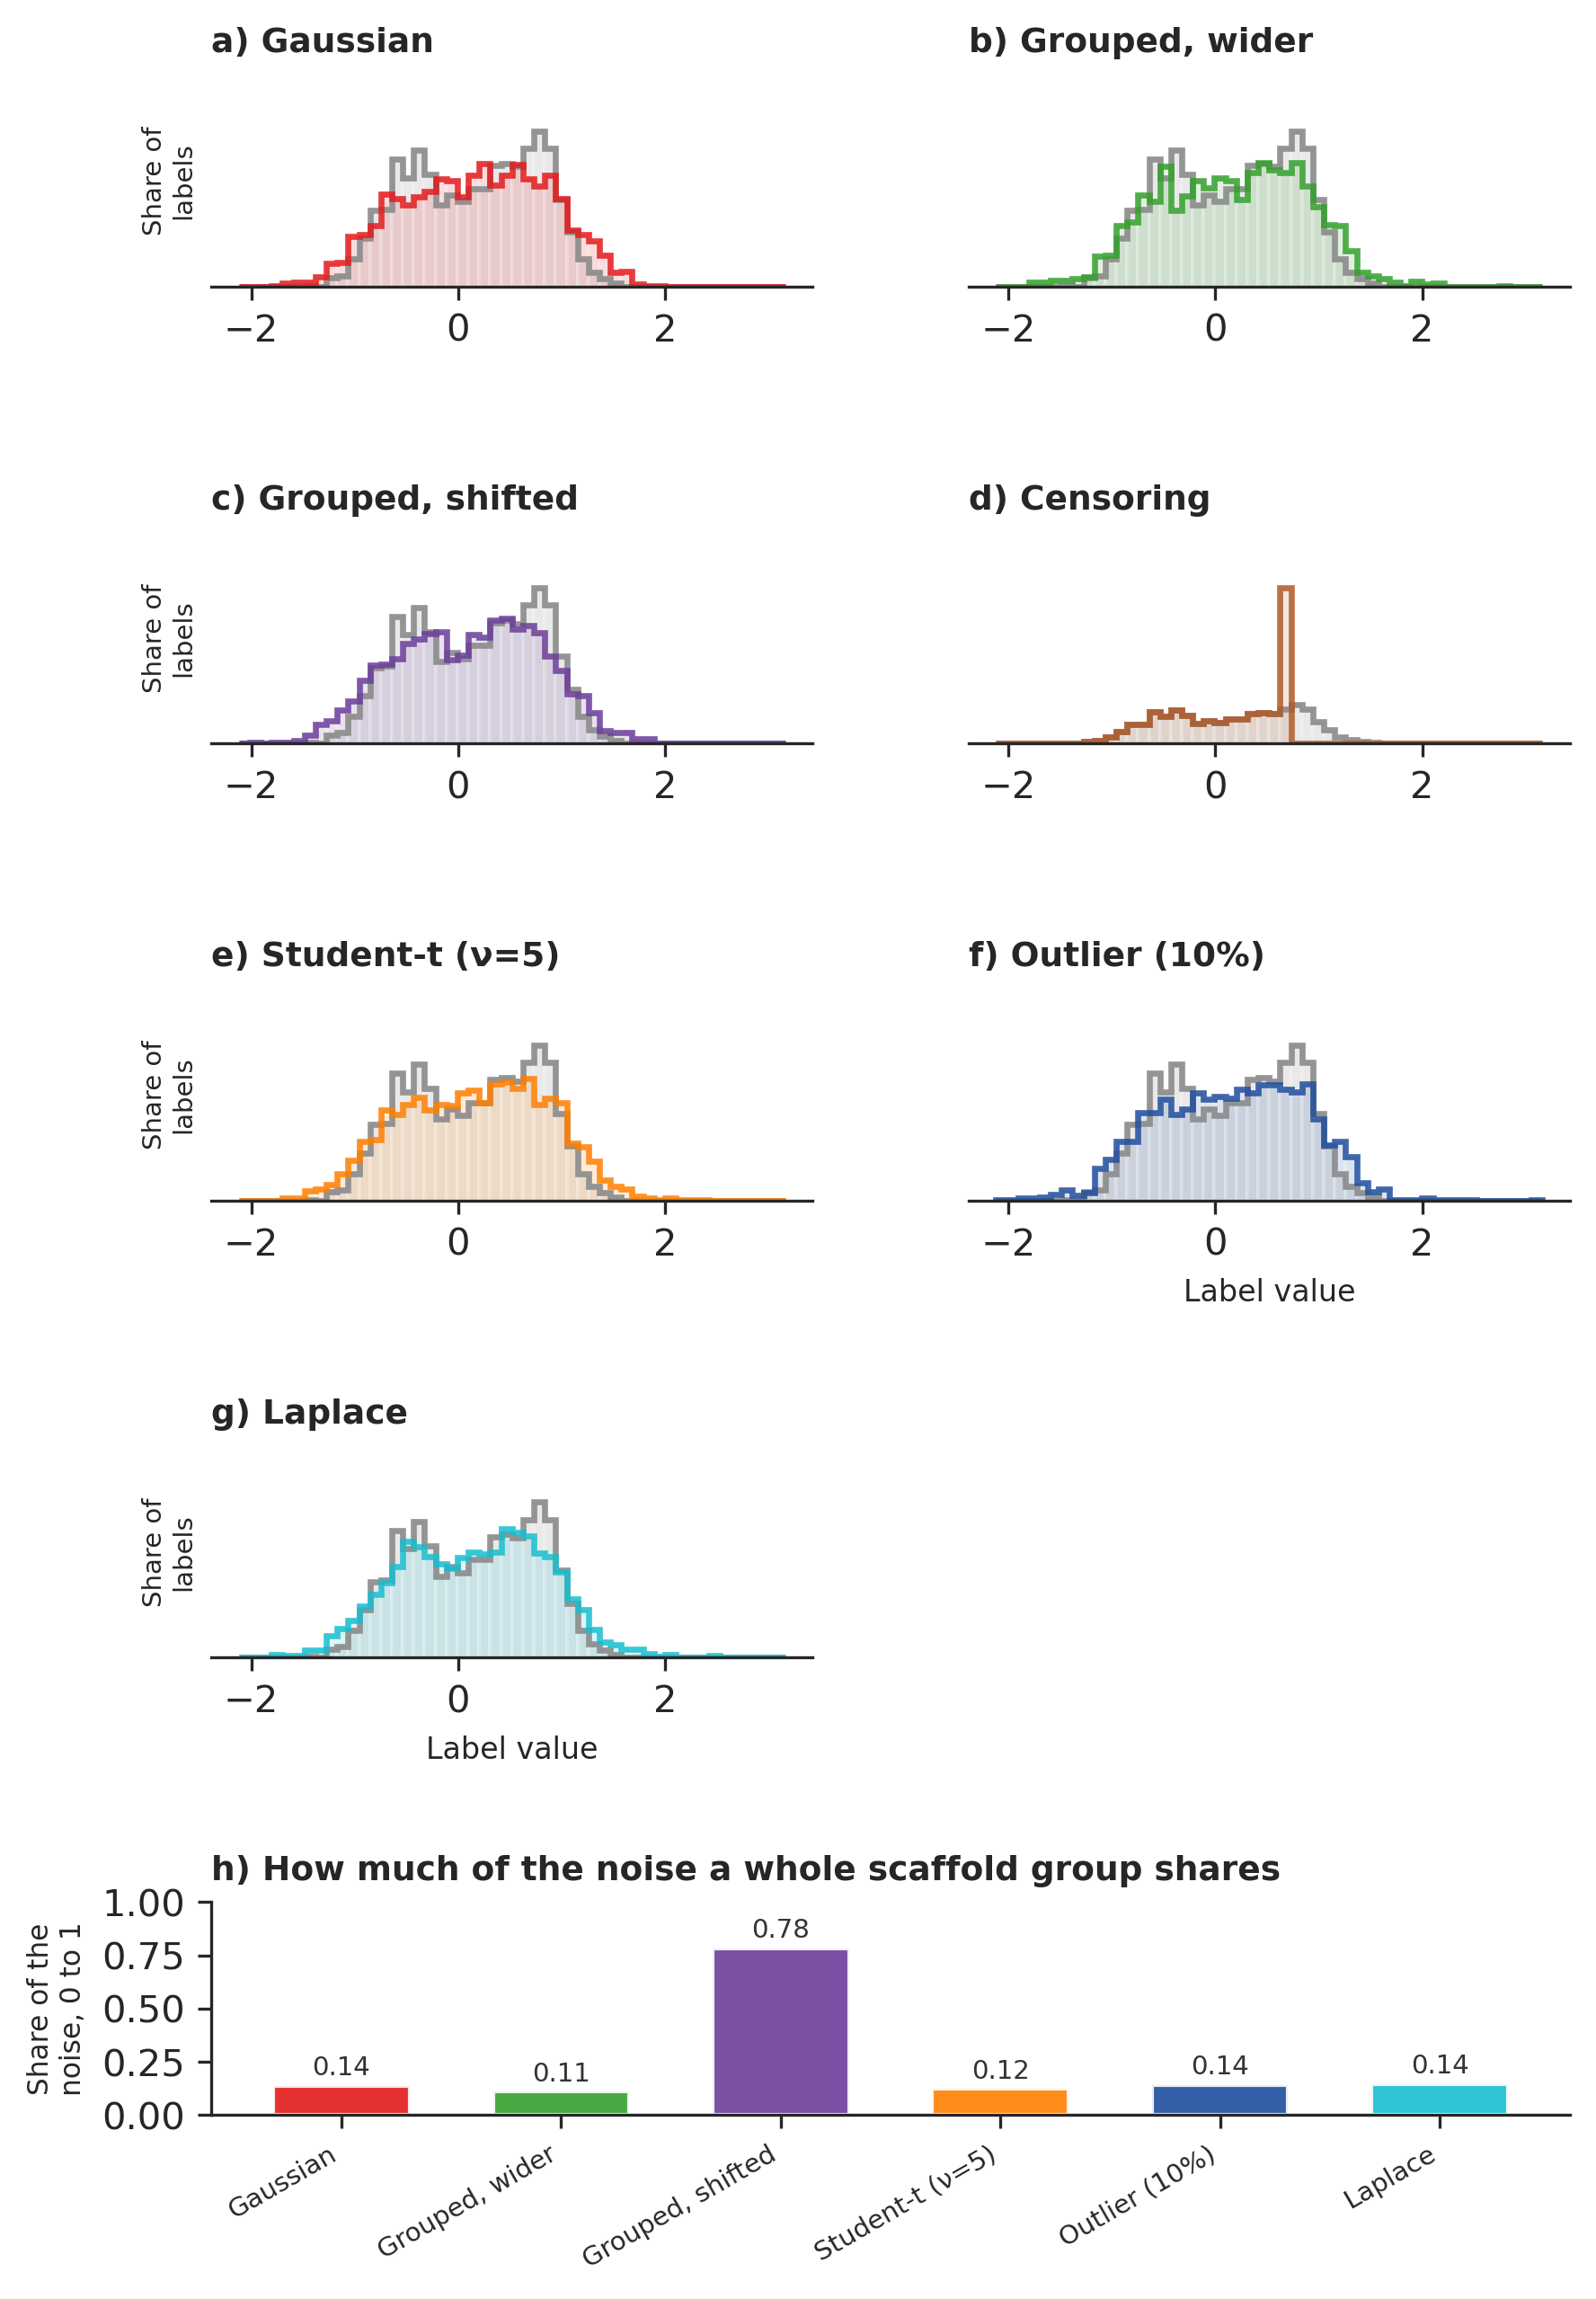
\includegraphics[width=\textwidth,height=0.72\textheight,keepaspectratio]{F1_noise_conditions.png}
\caption[Label distributions under the seven noise conditions.]{Label distributions under the seven noise conditions, for 2,000 synthetic labels in 40 random groups that stand in for scaffold families. a)--g) Clean (gray) and noised (color) labels at a noise level of 0.5 times the standard deviation of the clean labels (25\% of labels clipped under censoring). h) Standard deviation of the mean error within a group divided by that of all errors, for every condition except censoring; a value near 1 means a group's labels move together, and noise that ignores the groups gives about 0.14 with about 50 labels per group.}
\label{fig:noise_conditions}
\end{figure}

% TODO: review, needs manual review
At a set noise level, every condition except censoring delivers the same expected amount of noise over the training labels. These levels are defined as a fraction of the standard deviation of the clean training labels. The noise added to the label of molecule $i$ is
\begin{equation}
\epsilon_i = \frac{\tau}{G}\,s_i z_i,
\qquad
G = \sqrt{\frac{1}{n}\sum_{j=1}^{n} s_j^{2}}\;\;\sigma_z,
\label{eq:dose_matching}
\end{equation}
% TODO: review -- paper.tex text; novelty sentence removed because it conflicts with the Heid2023 sentence in the Chapter 3 introduction.
Here $\tau$ is the target standard deviation of the noise, equal to the noise level times the standard deviation of the clean training labels, and $z_i$ is
drawn from the condition's distribution at unit scale. The multiplier $s_i$ is $1$ for most
molecules and $\lambda = 3$ for those the condition affects, which are a random $10\%$ of molecules
under outlier and whole scaffold families covering $20\%$ of the training molecules under grouped-wider. The
constant $\sigma_z$ is the standard deviation of $z$, equal to $1$ for the Gaussian,
$\sqrt{\nu/(\nu-2)}$ for the Student-$t$ and $\sqrt{2}$ for the Laplace. The factor $G$ divides both
of these out, so that $\epsilon$ has standard deviation $\tau$ in expectation whatever the
distribution and whichever molecules are affected.

Grouped-shifted widens no molecule's error, and instead gives every scaffold family $g$ an offset of
its own,
\begin{equation}
\epsilon_i = \frac{\tau}{G}\left(\sqrt{\rho}\,b_{g(i)} + \sqrt{1-\rho}\,w_i\right),
\label{eq:grouped_shifted}
\end{equation}
with one draw $b$ per family and one draw $w$ per molecule. The two variances sum to $\tau^{2}$, and
the family offset carries a share $\rho$ of that total.

% TODO: No published figure exists for the fraction of scaffold families a difference between laboratories would cover, so we chose the $20\%$ above rather than sourcing it. - need to rephrase this 
% TODO: REVIEW MODIFICATION -- the parameter paragraph is now Table tab:noise_conditions. Every value and source in the table is from this paragraph; original kept below.
% We selected parameters from published measurement errors, wherever possible. As inter-laboratory error is estimated to be approximately three times intra-laboratory error, we set $\lambda = 3$ \citep{Avdeef2019}. \citet{Hampel2001} reports that $1-10\%$ of routine scientific data contains gross errors; we selected the upper bound of $10\%$. Laboratory identity accounts for $62\%$ of the variance in Caco-2 across 23 laboratories, prompting us to set $\rho = 0.62$ \citep{Bentz2013}. We took the Student-$t$ and Laplace shapes from the distributions fitted to repeated public bioactivity measurements \citep{Kruger2012}, and contaminated a fraction of the samples with a wider error according to Huber's contamination model \citep{huber1964robust}. As we found no published estimate of how large a share of a given dataset inter-laboratory differences affect, we chose to randomly select scaffolds until $20\%$ of the molecules had been covered. 
We selected the parameter values from published measurement errors wherever possible, and Table~\ref{tab:noise_conditions} notes where no published estimate exists.
\begin{table}[htbp]
\centering
\small
\begin{adjustbox}{max width=\textwidth,max totalheight=0.78\textheight}
\begin{tabular}{@{}P{0.15\linewidth}P{0.30\linewidth}P{0.17\linewidth}P{0.30\linewidth}@{}}
\toprule
\textbf{Condition} & \textbf{What It Changes} & \textbf{Value} & \textbf{Source for the Value} \\
\midrule
Gaussian & Shape: every label's error is Gaussian & -- & The standard assumption in noise-robustness studies \\
Student-$t$ & Shape: heavier tails than Gaussian & $\nu = 5$ & Distributions fitted to repeated bioactivity measurements \citep{Kruger2012} \\
Laplace & Shape: sharper peak and heavier tails than Gaussian & -- & As for Student-$t$ \citep{Kruger2012} \\
Outlier & Error $\lambda$ times wider on a random share of molecules (Huber's contamination model \citep{huber1964robust}) & $10\%$ of molecules; $\lambda = 3$ & $1$--$10\%$ of routine data contain gross errors, upper bound taken \citep{Hampel2001}; inter-laboratory error is about three times intra-laboratory error \citep{Avdeef2019} \\
Grouped-wider & Error $\lambda$ times wider on whole scaffold families & Families covering $20\%$ of the training molecules; $\lambda = 3$ & No published estimate of the share; $\lambda$ as for outlier \citep{Avdeef2019} \\
Grouped-shifted & Every scaffold family gets its own offset; no error is widened & $\rho = 0.62$ & Laboratory identity explains $62\%$ of the variance in log efflux ratio across 23 laboratories \citep{Bentz2013} \\
Censoring & Labels past a limit are set to the limit; the level is the fraction clipped & Set by the noise level & Censored labels in industrial assays \citep{Svensson2025} \\
\bottomrule
\end{tabular}
\end{adjustbox}
\caption[The seven noise conditions and their parameters.]{The seven noise conditions and their parameter values. $\nu$ is the number of degrees of freedom of the Student-$t$ distribution, $\lambda$ the widening factor (Equation~\ref{eq:dose_matching}) and $\rho$ the share of the noise variance carried by the scaffold-family offset (Equation~\ref{eq:grouped_shifted}). For censoring, the noise level is the fraction of labels clipped.}
\label{tab:noise_conditions}
\end{table}

% TODO: review, needs manual review (caption)

% CODE INPUT: heading added so the two \ref{sec:lnl_background} in Chapters 4 and 6 resolve. Section level and title need review; no prose written.
\subsection{Learning with Noisy Labels}\label{sec:lnl_background}
% ---- NOTES: Learning with noisy labels (planned section, no heading yet) ----
% Takeaway: LNL covers every method for training a model when some labels are wrong. Noise mitigation is the subset that changes the labels before training.
% Takeaway: no single method wins, and methods that compare a molecule with its neighbors fail where similarity fails.
% Paragraph 1: what LNL is.
% - Noise mitigation changes, drops or reweights the training labels once, before a model is trained. Any model can then be fitted to the result. Examples: removal, down-weighting, smoothing, relabeling, correction.
% - Noise-robust training leaves the labels and changes how the model trains. Examples: robust losses, noise-modeling layers, regularization, and reweighting inside the training loop (co-teaching, Meta-Weight-Net).
% - A sample-selection step taken out of its training loop and used only to delete molecules before a refit counts as noise mitigation.
% - Noise detection and noise estimation find or size noisy labels. They feed noise mitigation but are not LNL methods themselves.
% - Taxonomy of 62 deep-learning methods in five groups: robust architecture, robust regularization, robust loss function, loss adjustment, sample selection \citep{Song2022}.
% Paragraph 2: why no single method wins.
% - No free lunch: averaged over all problems, no learning algorithm beats another \citep{Wolpert1996, Wolpert1997}.
% - Chemistry analog: twelve algorithms on twelve bioactivity datasets with simulated experimental errors \citep{Cortes2015}.
% - Neighbor-based cleaning goes back to editing a training set by its nearest neighbors \citep{Wilson1972}. It relies on similar molecules having similar labels, which activity cliffs break.
% - QSAR models frequently fail to predict activity cliffs \citep{Dablander2023}.
% - Chapter 6 tests this.
% ---- END NOTES ----

% CODE INPUT
LNL covers every method for training a model when some of its labels are wrong, and we divide it into two parts. Noise mitigation changes, drops or reweights the training labels once, before any model is trained, so that any model can then be fitted to the result. Its methods include removal, down-weighting, smoothing, relabeling and correction, and Figure~\ref{fig:data_cleaning} shows how such a method is evaluated. Noise-robust training instead leaves the labels unchanged and alters how the model trains, through robust losses, noise-modeling layers, regularization, or reweighting inside the training loop, as in co-teaching \citep{Han2018} and Meta-Weight-Net \citep{shu2019metaweightnet}. A sample-selection step that is taken out of its training loop and used only to delete molecules before a refit counts as noise mitigation. Noise detection and noise estimation, which find noisy labels or estimate how many there are, feed into noise mitigation but are not LNL methods themselves. \citet{Song2022} sort 62 deep-learning methods into five groups, namely robust architecture, robust regularization, robust loss function, loss adjustment and sample selection.

% CODE INPUT: figure added from ~/Downloads/Data cleaning.png. It shows the example of QM9, a Bayesian model as the
% cleaner and a random forest scored by R^2. TODO: review -- keep here as the picture of noise mitigation, or move it.
\begin{figure}[!htbp]
    \centering
    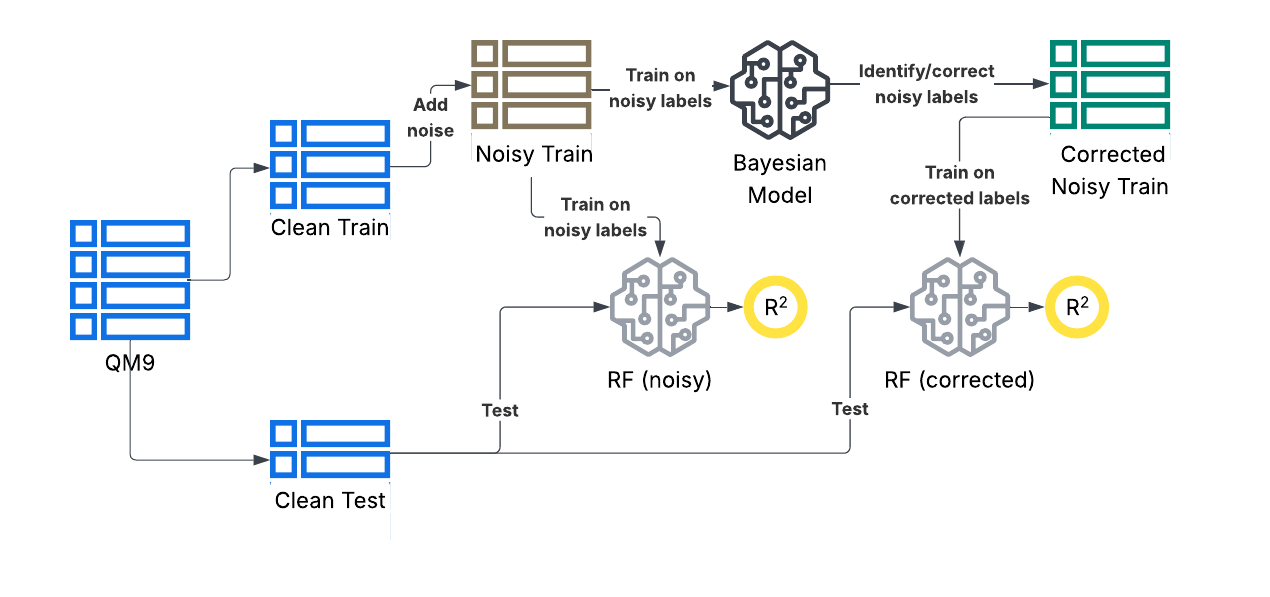
\includegraphics[width=0.95\textwidth,height=0.72\textheight,keepaspectratio]{figures_code_input/data_cleaning.png}
    \caption[Evaluation of a noise mitigation method.]{Evaluation of a noise mitigation method, with QM9 as the example. Noise is added to the training labels only. A random forest trained on the noisy labels is compared with one trained on labels corrected by a Bayesian model, and both are scored by $R^2$ on the clean test set.}
    \label{fig:data_cleaning}
\end{figure}
% CODE INPUT
% TODO: review, needs manual review (Cortes2015 details and the no-universal-solution sentence added from paper.tex)
No single method is expected to win, since averaged over all problems no learning algorithm outperforms another \citep{Wolpert1996, Wolpert1997}. The analog in chemistry is a study of twelve algorithms on twelve bioactivity datasets with simulated experimental errors at ten noise levels, which found that no single algorithm was best overall at maintaining predictive performance, and that some algorithms do better or worse at different levels of noise \citep{Cortes2015}. No single method can therefore be assumed to suit every dataset. Neighbor-based cleaning dates back to editing a training set by its nearest neighbors \citep{Wilson1972}, and it relies on similar molecules having similar labels, an assumption that activity cliffs break. QSAR models also frequently fail to predict activity cliffs \citep{Dablander2023}. Chapter~\ref{chap:flaws} tests the assumption that similar molecules have similar labels, and Chapter~\ref{chap:similarity} tests neighbor-based noise mitigation with the hybrid as the feature space.


\section{NoiseInject: A Benchmarking Framework}
% [notes moved to thesis_notes_moved.md]

% TODO: review, needs manual review
The noise conditions described above are implemented twice. NoiseInject, an open-source Python package, injects the noise on the three assay datasets and computes the robustness and uncertainty metrics, whereas QM9 uses a separate
pipeline, written in Python and Rust, that carries its own Rust implementation of the same conditions.
An automated check compares the two implementations before any experiment is run on the computing cluster. Because the random number generators of Rust and
NumPy produce different streams, the check compares statistics rather
than individual draws. On the same labels, groups and seeds, it compares the delivered noise, the
factor $G$, the median error, the number of badly corrupted labels and the number of molecules
affected.

\subsection{Package Description}\label{sec:noiseinject_pkg} % CODE INPUT: label added
% [notes moved to thesis_notes_moved.md]

% TODO: review, needs manual review
NoiseInject (version 1.0.0) evaluates model robustness and uncertainty calibration under artificial
label noise, for both regression and classification. It operates on arrays of labels and on the
predictions of any externally trained model, which makes it model-agnostic, and its core depends only
on NumPy, pandas, SciPy and scikit-learn. Results are returned as \texttt{pandas} data frames with one
row per noise level and one aggregate summary row. The software is available under an MIT license
and archived on Zenodo \citep{noiseinject}.

% TODO: review, needs manual review
\paragraph{Regression noise.} The regression injector specifies a noise shape (Gaussian, Student-$t$ or
Laplace) and a targeting rule (uniform, grouped-wider, grouped-shifted, outlier or censoring)
separately. Each named condition in the package is one combination of the two, together with its
parameters, and this name is recorded with every result. The package defines more settings
than Chapter~\ref{chap:robustness} uses, namely Student-$t$ distributions with $\nu \in \{3, 5, 10\}$ and outlier contamination of $1\%$,
$5\%$ and $10\%$ of molecules. It also defines an outlier variant in which the unselected molecules receive no
noise at all, rather than the base-scale noise of Equation~\ref{eq:dose_matching}.

% TODO: review, needs manual review
The requested noise is the root-mean-square noise $\tau$ in the units of the label, that is, the noise level times the standard deviation of the clean training labels. The
injector computes the per-molecule multipliers $s_i$ and solves for the scale $\tau / G$ in closed
form (Equation~\ref{eq:dose_matching}), so no calibration search is needed. A level of zero returns the
labels exactly unchanged. The affected molecules are selected with a second random number generator,
which is seeded separately from the noise draws and re-seeded on every call. As a result, the affected molecules are
the same at every noise level, including zero, while the noise draws themselves change. Under the
grouped-wider condition, whole scaffold families are added in random order until they cover as close as possible
to $20\%$ of the training molecules, because a fixed fraction of families
gives a very different fraction of molecules when family sizes are uneven.

% TODO: review, needs manual review
The censoring condition is parameterized by the fraction $f$ of labels clipped, and its limit is the $(1-f)$ quantile
of the clean training labels. On the training split, the censored
set is therefore exactly the $k = \mathrm{round}(fn)$ largest labels, whereas on any other split it consists of whichever
molecules lie past the training limit.

% TODO: review, needs manual review
Alongside the noisy labels, each injection returns a record of how they were produced. This record contains the target amount of noise, the factor
$G$, the solved scale, the delivered root-mean-square noise (in label units and as a fraction of the
clean label standard deviation), the mean of $\epsilon$, the fraction of molecules affected, the
number of groups and the largest share held by one group, and the random seeds. The injector also checks the delivered amount of noise.
Because the delivered amount is an estimate from a finite sample, it is compared against a band of three
standard errors,
\begin{equation}
\left|\frac{\hat{\tau}}{\tau} - 1\right| \le \max\!\left(3\sqrt{\frac{\kappa - 1}{4\,n_{\mathrm{eff}}}},\; 0.005\right),
\qquad
n_{\mathrm{eff}} = \frac{\left(\sum_i s_i^2\right)^2}{\sum_i s_i^4},
\label{eq:dose_tolerance}
\end{equation}
where $\hat{\tau}$ is the delivered root-mean-square noise and $\kappa$ is the sample kurtosis of the
unscaled draws $z$, bounded between 3 and 60. The effective count $n_{\mathrm{eff}}$ is the number of
independent contributions over which the delivered amount of noise averages, and it falls below $n$ when the noise is
concentrated on a few molecules. Under the grouped-shifted condition it is
$n_{\mathrm{eff}} = \left(\rho^2/g_{\mathrm{eff}} + (1-\rho)^2/n\right)^{-1}$, with
$g_{\mathrm{eff}} = \left(\sum_g n_g\right)^2 / \sum_g n_g^2$ for family sizes $n_g$. At
$\nu \le 4$ the Student-$t$ distribution has no fourth moment, so the standard error is instead
$1.3\,n_{\mathrm{eff}}^{\,2/\nu - 1}$, with the constant calibrated on the measured spread. A draw
outside the band raises a warning rather than an error. At three standard errors, a correct injector
falls outside the band on about $1\%$ of draws, and the delivered amount is recorded with the result
in either case.

% TODO: review, needs manual review
A second function of the package returns the noise scale that each molecule's region would receive, without drawing any noise.
We use it to score held-out molecules against the pattern of noise to which the training labels were exposed. Under the
uniform and grouped-shifted targeting rules this scale is the same for every molecule, so the package flags the result
as degenerate, because a rank correlation against a constant is undefined and must not be reported as zero.

% TODO: review, needs manual review
A separate injector sizes the noise against a unit supplied by the user rather than against the label standard
deviation. In the experiments implemented in the KIRBy repository, this unit is the standard deviation of a model's out-of-fold residuals on
the clean training labels, so that the noise is sized against the error the model already makes. Its
conditions either add Gaussian noise with variance equal to the level times the square of the unit, or move $2\%$,
$5\%$ or $10\%$ of labels by the level times the unit, with a random sign or always upward. They can also add
Gaussian noise whose standard deviation follows either a per-molecule covariate or a hidden
log-normal draw, and both of these are scaled to the same mean variance as the first condition.

% TODO: review, needs manual review
\paragraph{Classification noise.} The package provides six label-flipping strategies, namely uniform flips,
flip rates set by class frequency, asymmetric flip rates for binary tasks, a random flip rate for each sample,
a separate flip rate for each class, and flips directed by a confusion matrix. Because the realized
flip rate differs from the nominal flip probability under most of these strategies, a binary search
finds the flip probability that produces a target fraction of changed labels.

% TODO: review, needs manual review
\paragraph{Robustness metrics.} For regression, the package computes $R^2$, the root mean squared error (RMSE) and the mean absolute
error at every noise level. For classification, it computes accuracy, together with macro- and weighted-averaged precision, recall and F1
score and a per-class breakdown. Robustness is read from the
retention curve $\mathrm{ret}(x) = m(x)/m(0)$, where $m$ is a bounded metric for which higher values are better
($R^2$ for regression; accuracy, F1, precision or recall for classification) and $x$ is the noise
level. The primary summary is the normalized area under this curve,
\begin{equation}
\mathrm{AUC}_{\mathrm{norm}} = \frac{1}{x_{\max} - x_{\min}} \int_{x_{\min}}^{x_{\max}} \mathrm{ret}(x)\,\mathrm{d}x,
\label{eq:auc_norm}
\end{equation}
evaluated by the trapezoid rule. It is the mean fraction of clean performance retained across the
noise levels, lies approximately within $[0, 1]$, and is less directly correlated with clean-label $R^2$ than other robustness metrics we tested. A
secondary summary fits $\mathrm{ret}(x) \approx \exp\!\left(-(x/\tau_W)^{\beta}\right)$ to the curve. The shape parameter
$\beta$ separates curves that hold and then collapse ($\beta > 1$) from curves that fall early and
then plateau ($\beta < 1$), while $\tau_W$ sets the scale of the decay, and the fit requires at least four
noise levels. These two summaries replace the linear slope of performance against noise used in
earlier versions of NoiseInject, which misdescribed a nonlinear curve and was coupled to clean performance. The
package also reports the clean baseline and the retention at the highest noise level. A flag marks any
curve that falls below zero retention, and an optional threshold withholds the curve summaries for
models whose clean baseline is too low for a meaningful degradation.

% TODO: review, needs manual review
\paragraph{Uncertainty metrics.} For a model that returns a predicted standard deviation
$u_i$ for each sample, the package computes several metrics at each noise level. These are the Spearman correlation between $u_i$ and the
absolute error $|y_i - \hat{y}_i|$, the empirical coverage $\frac{1}{n}\sum_i \mathbb{1}\left[|y_i -
\hat{y}_i| \le k u_i\right]$ at $k = 1$ and $k = 2$ against Gaussian targets of $68.3\%$ and
$95.4\%$, the mean interval width $\frac{1}{n}\sum_i 2u_i$, and the expected calibration error (ECE),
\begin{equation}
\mathrm{ECE} = \sum_{b=1}^{10} \frac{|B_b|}{n}\,\left|\bar{u}_b - \overline{|y - \hat{y}|}_b\right|,
\label{eq:ece}
\end{equation}
computed over ten equal-count bins $B_b$ of $u$. All of these metrics are computed on the clean test labels. The Spearman
correlation between $u_i$ and the injected noise $|\epsilon_i|$ can only be computed where the noise
is known, which is on the corrupted molecules, so it requires a separate pair of inputs. It is reported
within each noise level, and a correlation pooled across all levels is returned separately. The pooled value
mostly reflects the fact that uncertainty and noise both rise with the level, so it
does not measure whether a model can identify which molecules are corrupted.

% TODO: review, needs manual review
Three optional wrappers produce $u_i$ from a point predictor. The first applies split-conformal prediction to any
scikit-learn-compatible model, optionally scaled by the label spread of each molecule's nearest
training neighbors. The second fits an exact Gaussian process with a Tanimoto or RBF kernel through \texttt{Gauche}
\citep{gauche}, and the third applies Monte Carlo dropout to any \texttt{PyTorch} network \citep{gal2016}. Example
notebooks and scripts cover regression and classification from start to finish.


\section{Evaluation Methodology}
% [notes moved to thesis_notes_moved.md]

% TODO: review, needs manual review
Chapter~\ref{chap:robustness} reports predictive performance as $R^2$ on held-out molecules and robustness as \aucnorm{} (Equation~\ref{eq:auc_norm}). Chapters~\ref{chap:flaws} to~\ref{chap:similarity} state the metric used for each dataset where it is introduced.

\section{Conclusions}

% ---- NOTES: Conclusions ----
% Takeaway: a predictor is a representation paired with a model; Chapter 3 asks which of the two governs how badly a predictor degrades under label noise.
% Paragraph 1: 3-4 sentences.
% - Sentence 1: both halves of a predictor, the representation and the model, have now been introduced.
% - Sentence 2: real assay noise is not independent, identically distributed or symmetric. The artificial noise model has seven conditions. LNL methods have been set out, with noise mitigation as the subset that acts on the labels.
% - No single LNL method wins on every dataset.
% - Sentence 3: NoiseInject injects the conditions and reports robustness and uncertainty metrics. The evaluation section fixes the splits and metrics.
% - Sentence 4: Chapter 3 asks whether the representation or the model architecture governs how badly a predictor degrades under label noise. Point to Chapter 1 for its four questions.
% - Optional: the representations, similarity definitions and noise conditions are reused in Chapters 4 to 6.
% ---- END NOTES ----

% CODE INPUT
% TODO: review, needs manual review -- splits text not yet written; notes in thesis_notes_moved.md
This chapter has introduced both halves of a predictor, namely the representation and the model. Because real assay noise is not independent, identically distributed or symmetric, our artificial noise model comprises seven conditions. We have also set out the methods for LNL, of which noise mitigation is the subset that acts on the labels, and noted that no single method wins on every dataset. NoiseInject injects these noise conditions and reports the robustness and uncertainty metrics, and the section on evaluation methodology fixes the metrics. Chapter~\ref{chap:robustness} asks whether the representation or the model architecture governs how strongly a predictor degrades under label noise, through the four questions set out in Chapter~\ref{chap:intro}. The representations, similarity definitions and noise conditions introduced here are reused in Chapters~\ref{chap:flaws} to~\ref{chap:similarity}.

